\documentclass[12pt, danish]{beamer}

\usepackage[danish]{babel}
\usepackage[utf8x]{inputenc}
\usepackage{graphics}
\usepackage{srcltx}
\usepackage{float}
\usepackage{layout}
\usepackage{listings}

\title{Siberian Transport System}
\author{Troels Henriksen, Shantanu Bala, Jesper Tved}

\mode<presentation>
{
  %\usetheme{Frankfurt}
  \usetheme{Warsaw} 
  \definecolor{uofsgreen}{rgb}{.125,.5,.25}
  \definecolor{natvidgreen}{rgb}{.196,.364,.239}
  \definecolor{kugrey}{rgb}{.4,.4,.4}
  \usecolortheme[named=uofsgreen]{structure}
  \usefonttheme[onlylarge]{structuresmallcapsserif}
  \usefonttheme[onlysmall]{structurebold}
}

\usenavigationsymbolstemplate{} % fjern navigation

\setcounter{tocdepth}{1}

\def\height{0.6\paperheight}
\def\width{0.9\linewidth}

\setlength{\marginparwidth}{1pt}
\setlength{\hoffset}{1pt}

\begin{document}

\begin{frame}
\titlepage
\end{frame}

\begin{frame}
\frametitle{Scope}

Russia has an extensive raw materials industry located in remote
Siberian locations.  Poor conditions make transport times by truck
unpredictable.  It is necessary to have automatically updated
information about the whereabouts of the truck fleet.

\pause

Each truck reports its location to a central server when possible.
The server aggregates the information and makes it available for
decision making.

\pause

The system is solely concerned with the state of the trucking fleet,
and does not do freight tracking or make any kind of business logic
decisions on its own.  Also, it is a one-way communication system,
other means must be employed to contact the trucks.  A data
interchange mechanism will be designed that allows other systems to
receive information from STS.

\end{frame}

\begin{frame}
\begin{center}
\frametitle{Context diagram}
  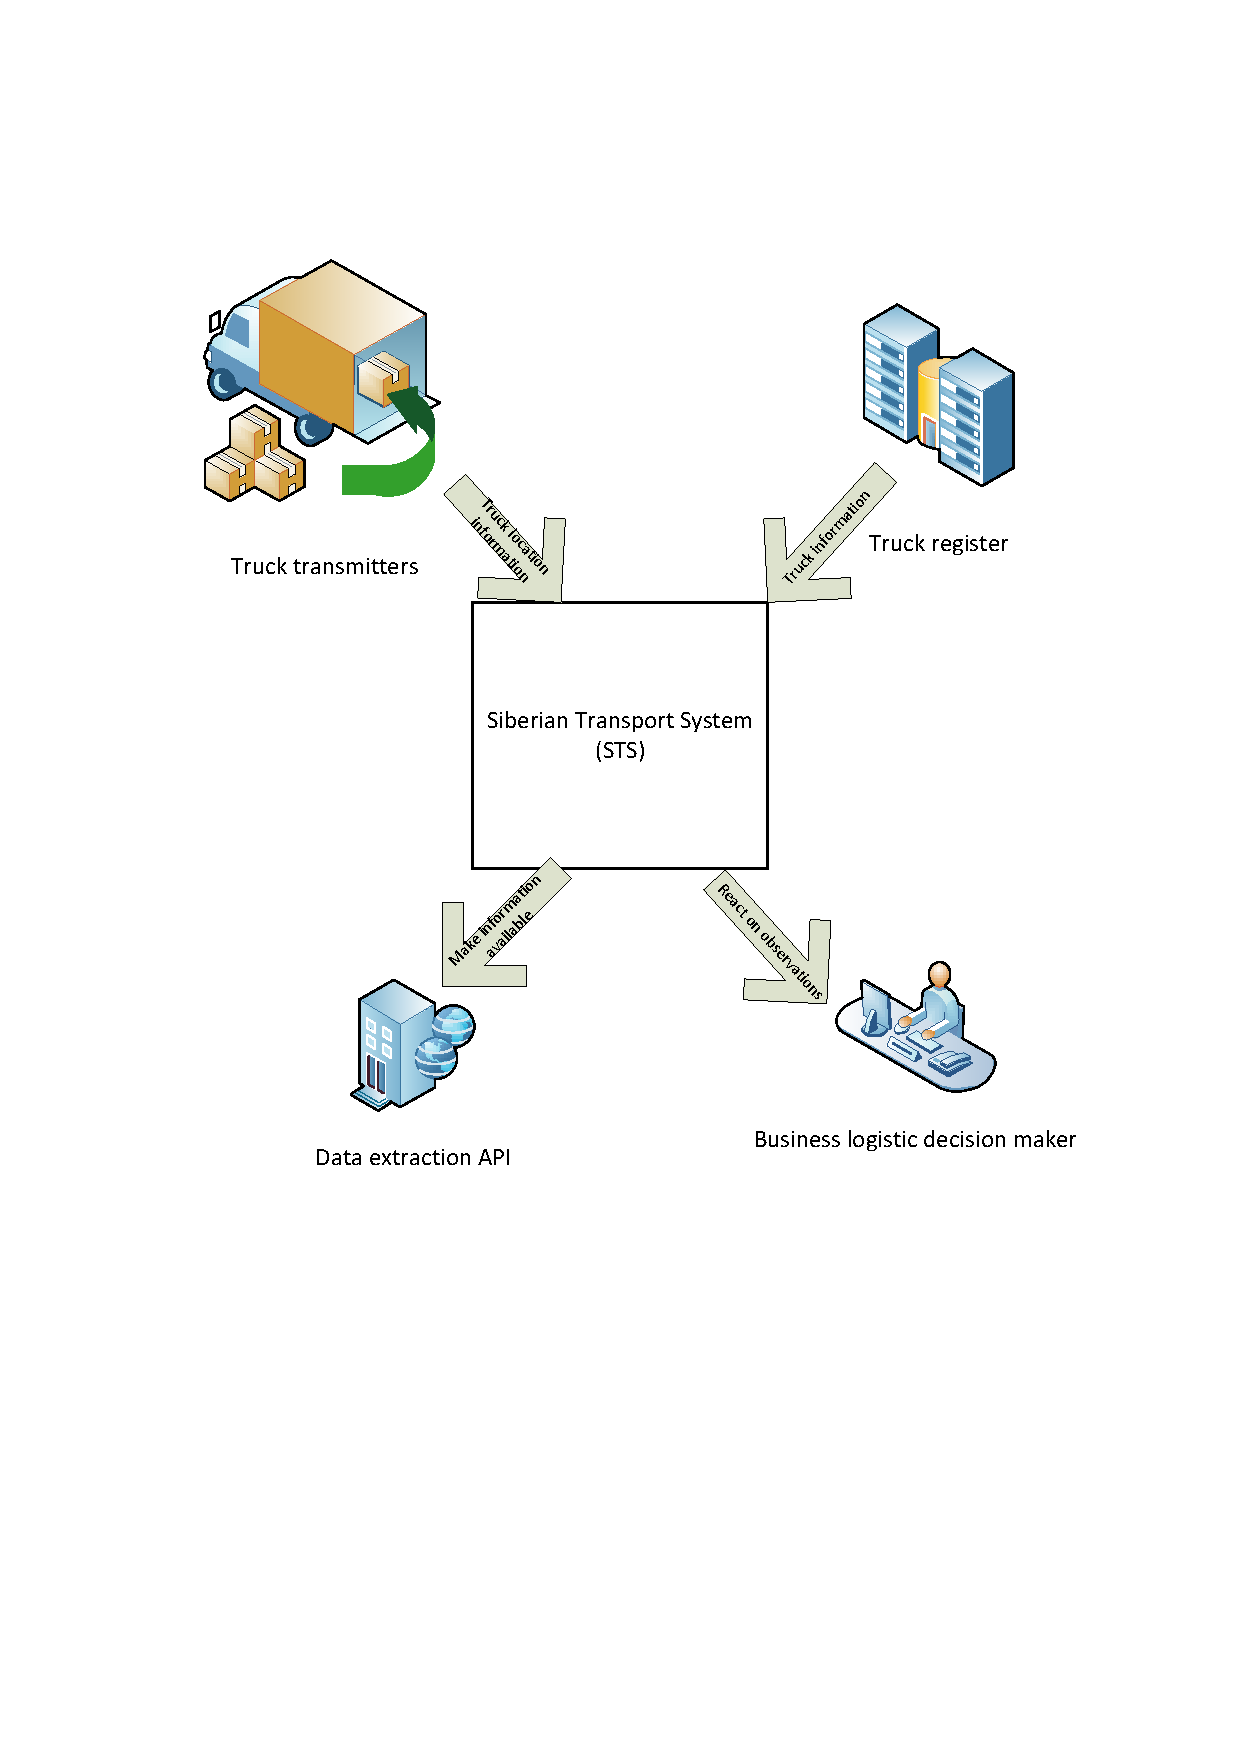
\includegraphics[height=12cm]{sts_context_view}\\
\end{center}
\end{frame}

\end{document}
